% Свежая версия шаблона здесь <https://www.overleaf.com/read/sqvxbnhgxxdm>
\documentclass[14pt,a4paper,report]{ncc}
\usepackage[a4paper, mag=1000, left=2.5cm, right=1cm, top=2cm, bottom=2cm, headsep=0.7cm, footskip=1cm]{geometry}
\usepackage[utf8]{inputenc}
\usepackage[english,russian]{babel}
\usepackage{indentfirst}
\usepackage[dvipsnames]{xcolor}
\usepackage[colorlinks]{hyperref}
\usepackage{listings} 
\usepackage{caption}
\usepackage{amssymb}
\usepackage{tcolorbox}
\DeclareCaptionFont{white}{\color{white}} %% это сделает текст заголовка белым
%% код ниже нарисует серую рамочку вокруг заголовка кода.
\usepackage{color} %% это для отображения цвета в коде
\DeclareCaptionFormat{listing}{\colorbox{gray}{\parbox{\textwidth}{#1#2#3}}}
\captionsetup[lstlisting]{format=listing,labelfont=white,textfont=white}
\lstset{% Собственно настройки вида листинга
inputencoding=utf8, extendedchars=\true, keepspaces = true, % поддержка кириллицы и пробелов в комментариях
language=C++,            % выбор языка для подсветки (здесь это Pascal)
numberstyle =\tiny
basicstyle=\small\sffamily, % размер и начертание шрифта для подсветки кода
keywordstyle =\color{ForestGreen},
numbers=left,               % где поставить нумерацию строк (слева\справа)
numberstyle=\tiny,          % размер шрифта для номеров строк
stepnumber=1,               % размер шага между двумя номерами строк
numbersep=5pt,              % как далеко отстоят номера строк от подсвечиваемого кода
backgroundcolor=\color{white}, % цвет фона подсветки - используем \usepackage{color}
showspaces=false,           % показывать или нет пробелы специальными отступами
showstringspaces=false,     % показывать или нет пробелы в строках
showtabs=false,             % показывать или нет табуляцию в строках
frame=single,               % рисовать рамку вокруг кода
tabsize=2,                  % размер табуляции по умолчанию равен 2 пробелам
captionpos=t,               % позиция заголовка вверху [t] или внизу [b] 
breaklines=true,            % автоматически переносить строки (да\нет)
breakatwhitespace=false,    % переносить строки только если есть пробел
escapeinside={\%*}{*)}      % если нужно добавить комментарии в коде
}

\begin{document}
% Переоформление некоторых стандартных названий
%\renewcommand{\chaptername}{Лабораторная работа}
\def\contentsname{Содержание}

% Оформление титульного листа
\begin{titlepage}
\begin{center}
\textsc{ФГОУ ВО Уральский Федеральный Университет \\ имени первого Президента России Б.Н.Ельцина\\[5mm]
Физико-технологический институт\\[2mm]
Кафедра теоретической физики и прикладной математики}

\vfill

\textbf{ОТЧЁТ ПО ЛАБОРАТОРНОЙ РАБОТЕ №7\\[3mm]
«Моделирование объединенной атомной и спиновой динамики системы магнитных частиц»\\[6mm]
}
\end{center}

\hfill
\begin{minipage}{.5\textwidth}
Студент:\\[2mm] 
Вялова С.А.\\
группа: ФтМ-170403 \\[5mm]

Преподаватель:\\[2mm] 
д.ф.-м.н., профессор\\
Мазуренко Владимир Владимирович\\[5mm]

Консультант:\\[2mm] 
н.с.\\
Сотников Олег Михайлович\\

\end{minipage}%
\vfill
\begin{center}
\today  \\
%\theyear\, г.
 Екатеринбург.
\end{center}
\end{titlepage}

% Содержание
\tableofcontents
\newpage
\chapter{Моделирование объединенной атомной и спиновой динамики системы магнитных частиц}
\section{Цель работы}


Разработка компьютерной программы для моделирования объединенной атомной и спиновой динамики системы частиц с дефектами типа вакансий, используя метод Монте Карло, а именно алгоритм Метрополиса.
\


В ходе выполнения работы необходимо реализовать следующие пункты:
\
\begin{itemize}
\item провести моделирования спиновой и молекулярной динамики системы, в которой атомы испытывают колебания вблизи положений равновесия;
\item проанализировать поведение системы в зависимости от параметров $J_0$ и $r_c$;
\end{itemize}

\

\newpage\section{Теоретическая часть }
\subsection{Потенциал Леннарда-Джонса}
%text
Потенциал Леннарда-Джонса представляет собой простую модель парного взаимодействия неполярных молекул, описывающая зависимость энергии взаимодействия двух частиц от расстояния между ними.
Потенциал был предложен Леннардом-Джонсом первоначально для исследования термодинамических свойств инертных газов. Наиболее часто используется так называемый (6-12)-потенциал Леннарда-Джонса, записанный в форме 
\
\begin{equation}
 U = 4 \cdot \varepsilon \cdot [(\sigma/r)^{12} - (\sigma/r)^{6}  ] ,
 \end{equation} 
где $\varepsilon$ - глубина потенциальной ямы, $\sigma$ - значение расстояния между частицами, при котором потенциал равен нулю. Шестая степень убывания отвечает электростатическому диполь-дипольному и дисперсионному притяжению; двенадцатая степень убывания потенциала моделирует достаточно жесткое отталкивание и выбрана из соображений математического удобства.
\
\subsection{Алгоритм Метрополиса}
Таким образом, у нас есть двумерная система частиц, которые могут смещаться случайным образом в пределах некой окружности вблизи начального положения, но так, что можно достичь состояния с любой энергией за конечное количество шагов (условие эргодичности). Для конечных температур следует ожидать, что энергия системы должна флуктуировать вокруг некоторого равновесного значения. Чтобы вычислять термодинамические величины необходимо разыгрывать состояния таким образом, чтобы система пришла к состоянию равновесия за какое-то разумное время. Для этих целей и служит Алгоритм Метрополиса. Его можно разбить на следующие шаги:

\vspace{8mm}
\begin{enumerate}
\item сгенерировать начальную конфигурацию системы $\alpha_k$;
\item выбрать $i$-ую частицу и сместить ее, сгенерировав тем самым пробное состояние системы  $\alpha_i$;
\item вычислить энергию нового состояния $E_i$;
\item если $E_k>E_i$, принять новое состояние системы;
\item если $E_i>E_k$, принять новое состояние с вероятностью:\\
$R=exp(\Delta E/kT)$;
\begin{itemize}
\item выбрать случайное число $0\le r\le 1$
\item положить состояние 
\[
\alpha_{k+1}=
\begin{cases}
\alpha_k, & \text{если $R\ge r$;} \\
\alpha_i, & \text{если $R<r$.}
\end{cases}
\]
\end{itemize}
\item вычислить нужные величины в состоянии $\alpha_{k+1}$, взять его за начальное и повторять с пункта 2 нужное количество шагов.
\end{enumerate}


%\caption{Зависимость температуры системы от шага по времени.}

\subsection{Описание  методов}
%text
В ходе работы необходимо исследовать спиновую и молекулярную динамику систем частиц, колеблющихся вблизи положений равновесия. Для этого был видоизменен программный код для программы моделирования квазидинамики частиц, реализованной при использовании алгоритма Метрополиса.
\

Частицы выбранных систем взаимодействуют через потенциал Леннарда-Джонса, спиновая динамика системы описывается гамильтонианом Гейзенберга. Для молекулярной динамики необходимо задать начальные координаты частиц (в данной работе выбирается начальное положение частиц в виде треугольной конфигурации решетки), параметр $\sigma$, соответствующий основному состоянию треугольной решетки, размеры которой по горизонтали $L_x$, по вертикали $L_y=\sqrt{\frac{\sqrt(3)}{2}}L_x$, а также параметр $\epsilon$. Для реализации спиновой динамики необходимо задать произвольным образом начальные углы отклонения $\theta_i$ и $\phi_i$ для каждого спина, где $i$ - номер спина.
\



Пусть $L_x$ - ширина треугольной решетки, $n_c$ - число частиц в каждой строке или столбце. Столбцы треугольной решетки отстоят друг от друга на $a={L_x}/{n_c}$, а каждую строку разделяет расстояние ${\frac{\sqrt{3}}{2}} a$. В каждой строке узлы смещены на $\frac{a}{2}$ относительно предыдущей строки. Высота треугольной решетки составляет $L_y={\frac{\sqrt{3}}{2}} L_x$, а общее число частиц в системе составляет $n={n_c}^2$. 
\

После чего, для поиска глобального минимума системы, запускается квазидинамика системы, реализованная при использовании алгоритма Метрополиса.
\ 

Энергия решетки вычисляется через потенциал Леннарда-Джонса следующим образом:
\begin{equation}
E=4 \varepsilon \sum\limits_{i=1}^N \sum\limits_{s=i+1}^N{ [(\sigma/\vec{r}_{is})^{12} - (\sigma/\vec{r}_{is})^{6}]+\sum\limits_{ij}^N{J_{ij}(r_{ij})(\vec{S_i} \cdot \vec{S_j})}  }
\end{equation}
\

На каждом шаге алгоритма Метрополиса для каждой частицы системы инициируется малое смещение $dx_i$ и $dy_i$, выбранное произвольным образом в промежутке $[-dr, dr]$ и реализуется пробное смещение $i$-й частицы системы. Одновременно с этим инициируется малые смещения спинов $dx$, $dy$, $dz$ выбранные произвольным образом в промежутке $[-dr, dr]$. После этого считается энергия пробного состояния системы, и в зависимости от её изменения в большую или меньшую сторону от предыдущей энергии состояния, выбирается решение, принять ли данное пробное состояние или оставить систему в предшествующем смещению состоянии.

\

\subsection{Результаты моделирования квазидинамики при использовании алгоритма Метрополиса}
Система задана со следующими параметрами:
\begin{itemize}
\item Линейные размеры системы по горизонтали $L_x=7$, линейные размеры системы по вертикали $L_y=\frac{\sqrt{3}}{2}L_x$;
\item число частиц $n=64$;
\item $\sigma=1,047$;
\item температурный множитель $kT=0,00005$;
\item число шагов алгоритма Метрополиса $N=10000$;
\item $\epsilon=0.0031$;
\item $|J_0|=0,01$;
\item $r_c=2$;
\item $dr=0,001$;
\end{itemize}

Рассмотрим результаты моделирования системы с ферромагнитным характером взаимодействия между спинами. Начальное состояние системы представлено на рисунке \ref{ris:image1}. Как видно, в начальный момент времени спины разупорядочены.
\

\begin{figure}[b]
\center{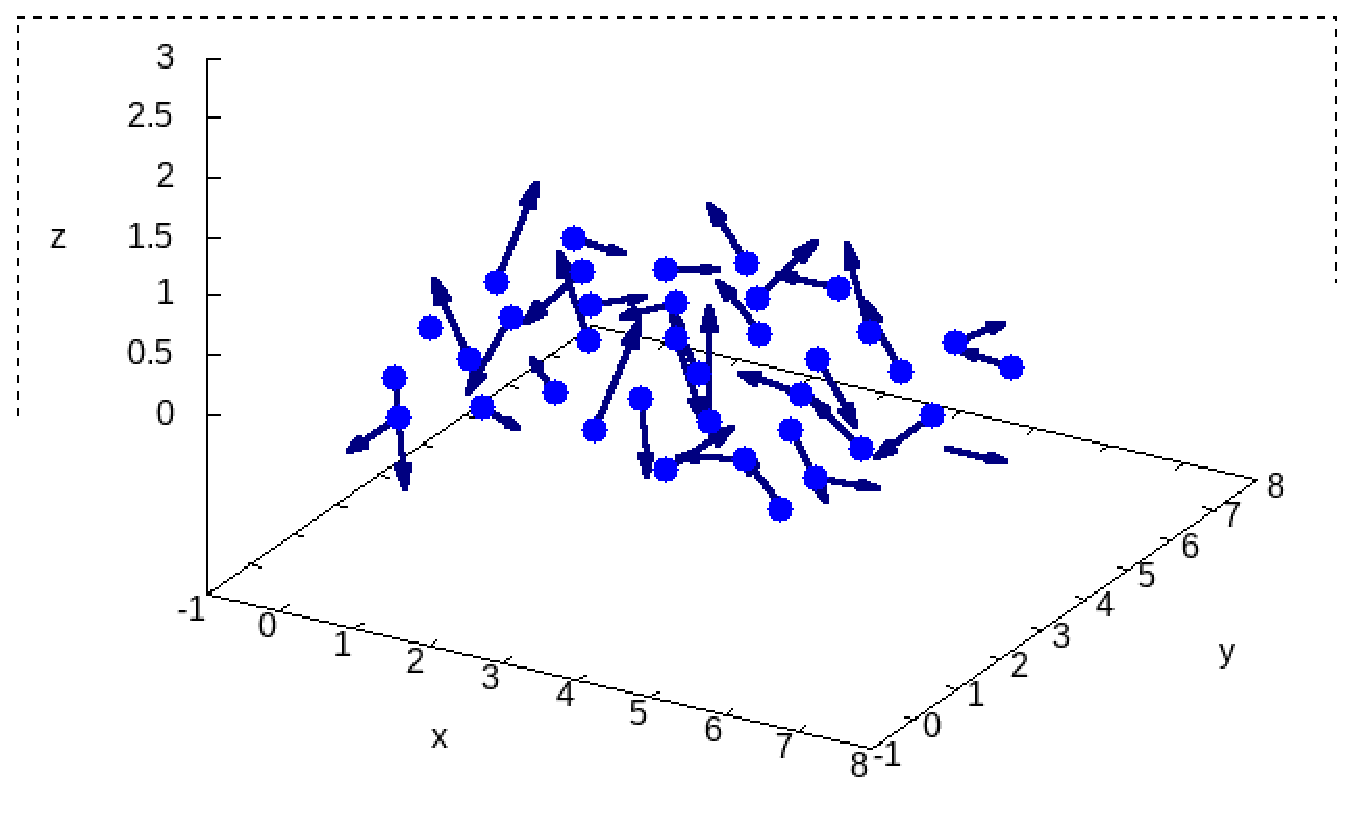
\includegraphics[width=0.5\linewidth]{pictures/INIT}}
\caption{Проекции спинов в начальный момент времени.).}
\label{ris:image1}
\end{figure}
\ref{ris:image1}. 


\
\begin{figure}[h]
\begin{minipage}[h]{0.49\linewidth}
\center{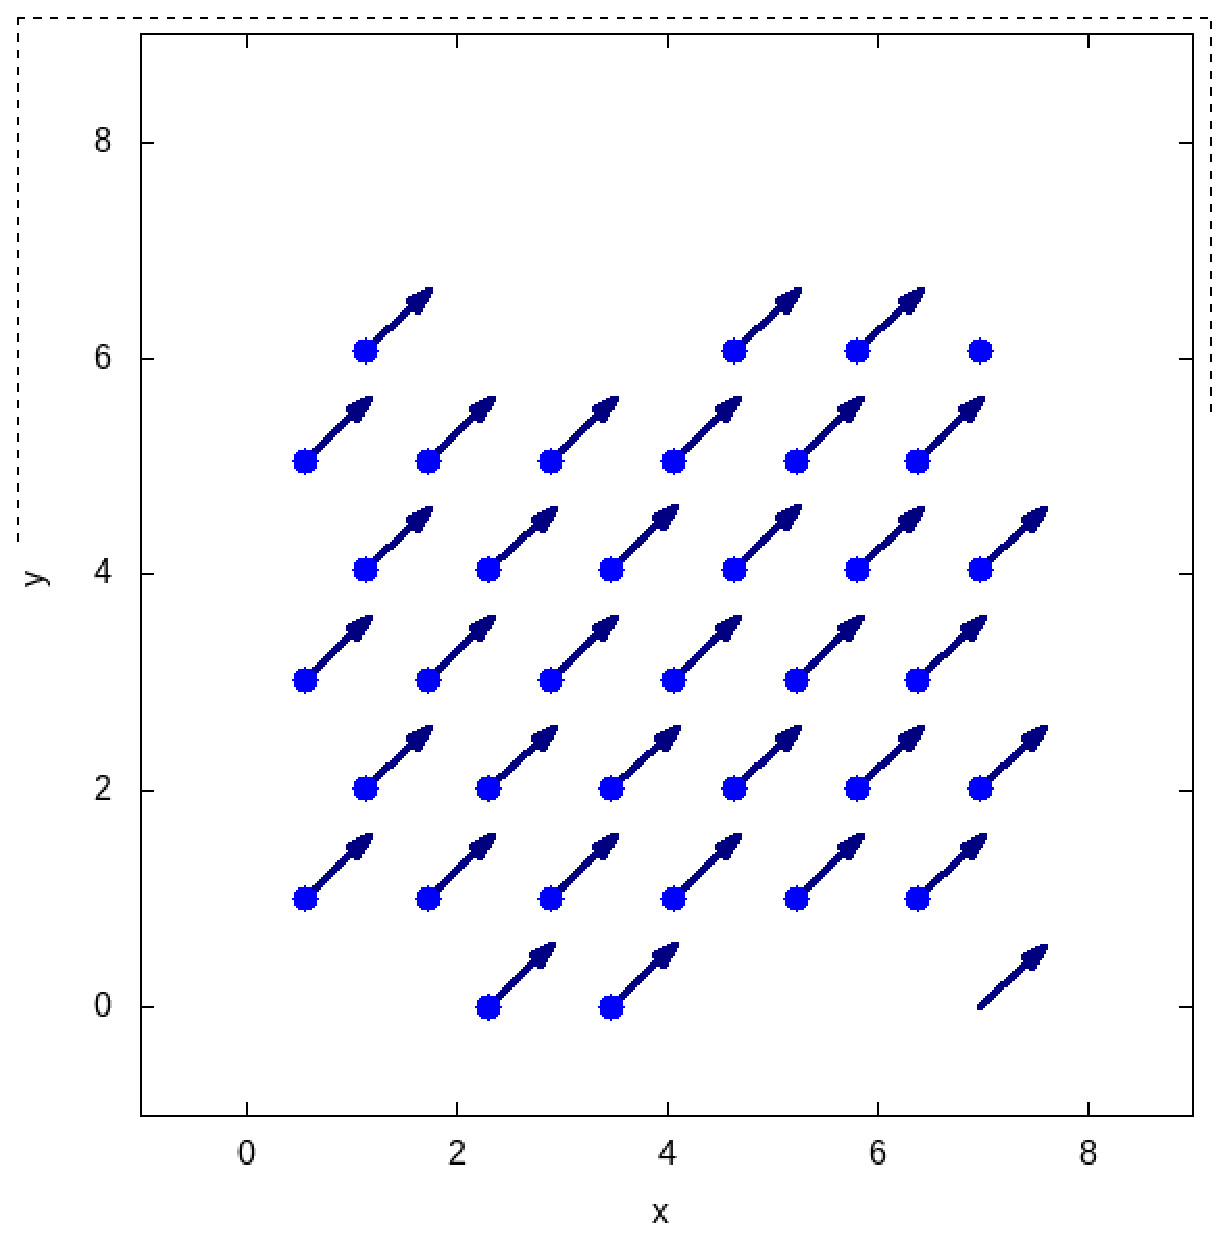
\includegraphics[width=0.5\linewidth]{pictures/FM01} \\ а)}
\end{minipage}
\hfill
\begin{minipage}[h]{0.49\linewidth}
\center{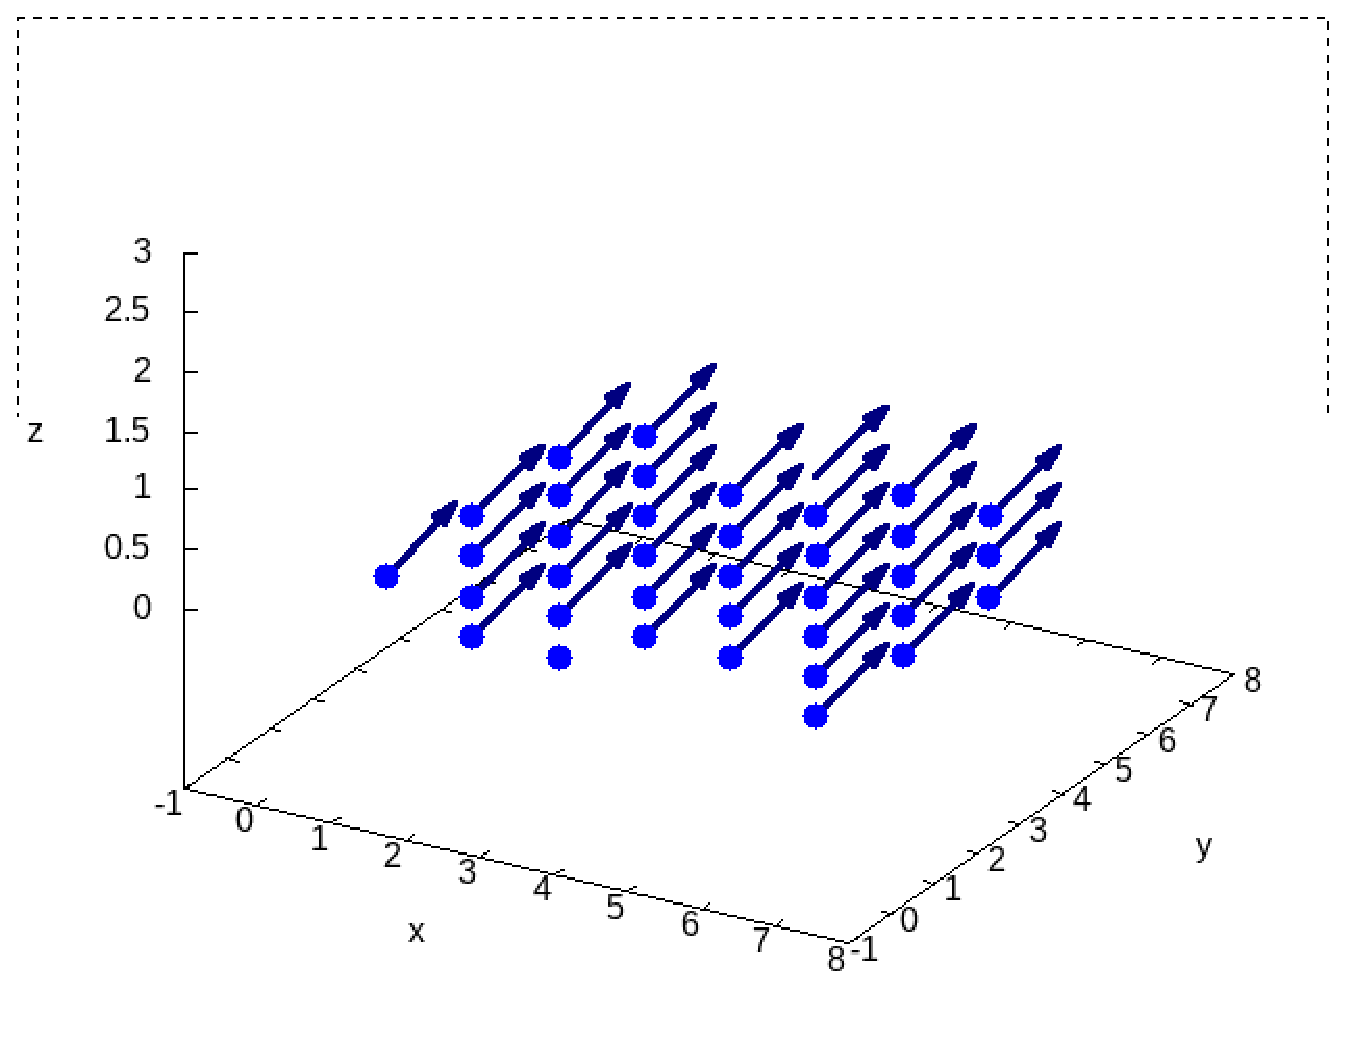
\includegraphics[width=0.5\linewidth]{pictures/FM013D} \\ б)}
\end{minipage}
\caption{Конечное состояние системы, в которой взаимодействие между спинами носит ферромагнитный характер $J_0=-0.01$, $r_c=2$.}
\label{ris:image2}
\end{figure}


Спины, как и ожидалось, выстроились параллельно друг другу (рисунок \ref{ris:image2}). Угол между осью $z$ и каждым спином равен $\pi/2$.
Графики зависимостей энергии системы от шага моделирования изображены на рисунке \ref{ris:image5}. Как видно из графиков энергии, система приходит в положение равновесия с меньшей энергией по мере упорядочения спинов.
\



Рассмотрим случай антиферромагнитного упорядочения, получим картину расположения спинов и частиц, представленную на рисунке \ref{ris:image5}. Спины выстроились антипараллельно.

\
\begin{figure}[h]
\begin{minipage}[h]{0.49\linewidth}
\center{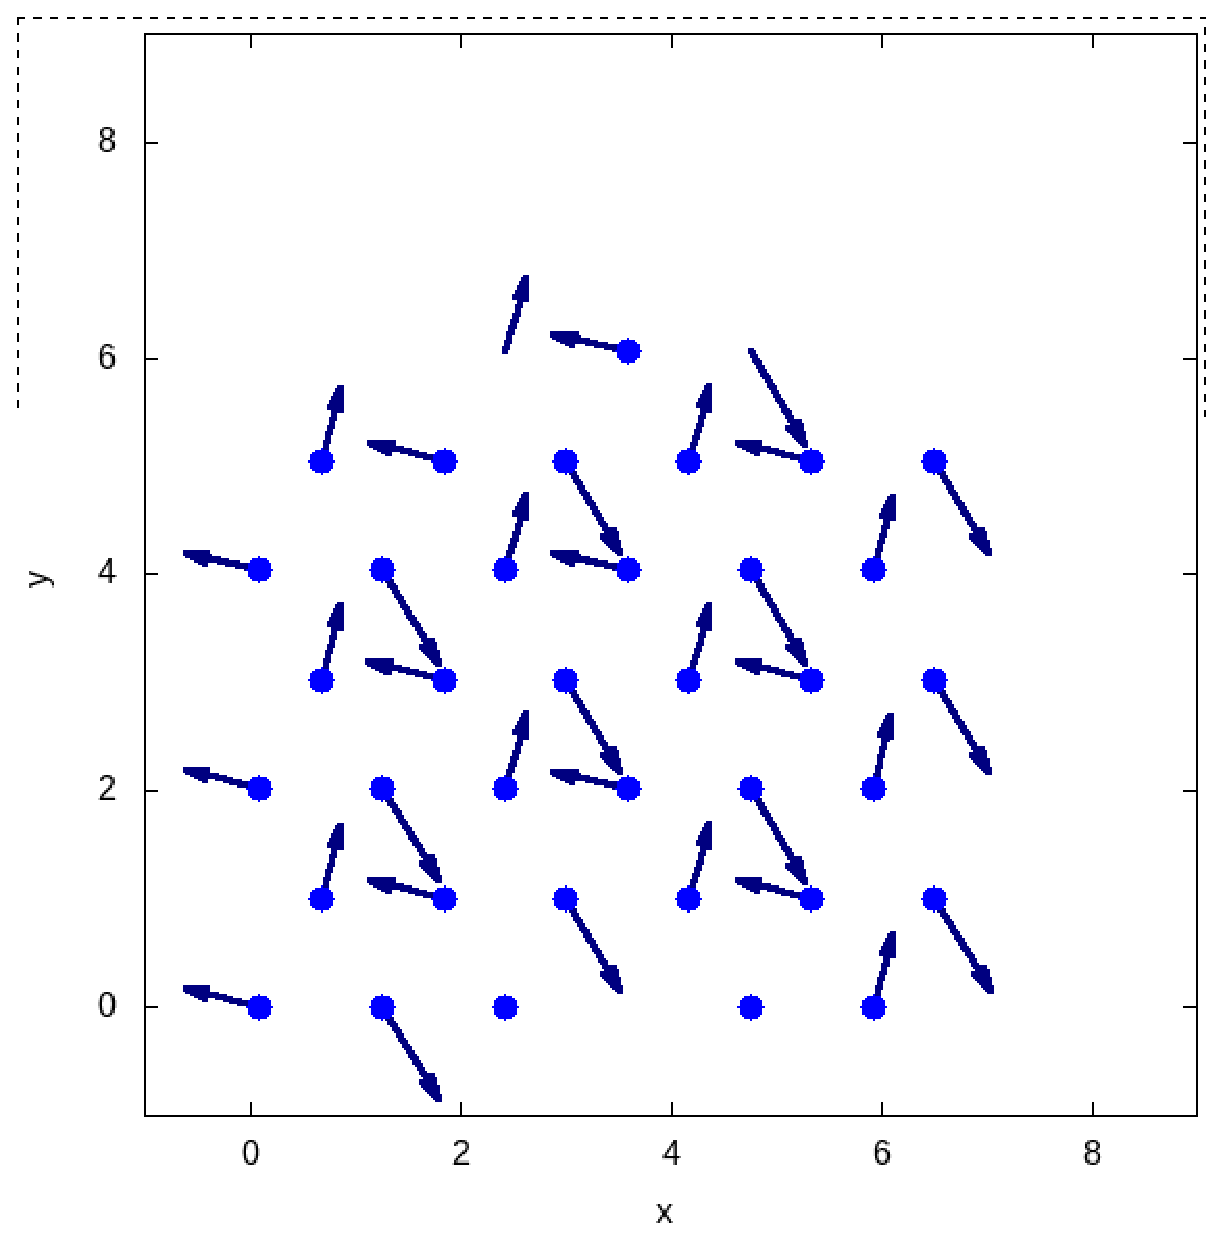
\includegraphics[width=0.5\linewidth]{pictures/AFM01} \\ а)}
\end{minipage}
\hfill
\begin{minipage}[h]{0.49\linewidth}
\center{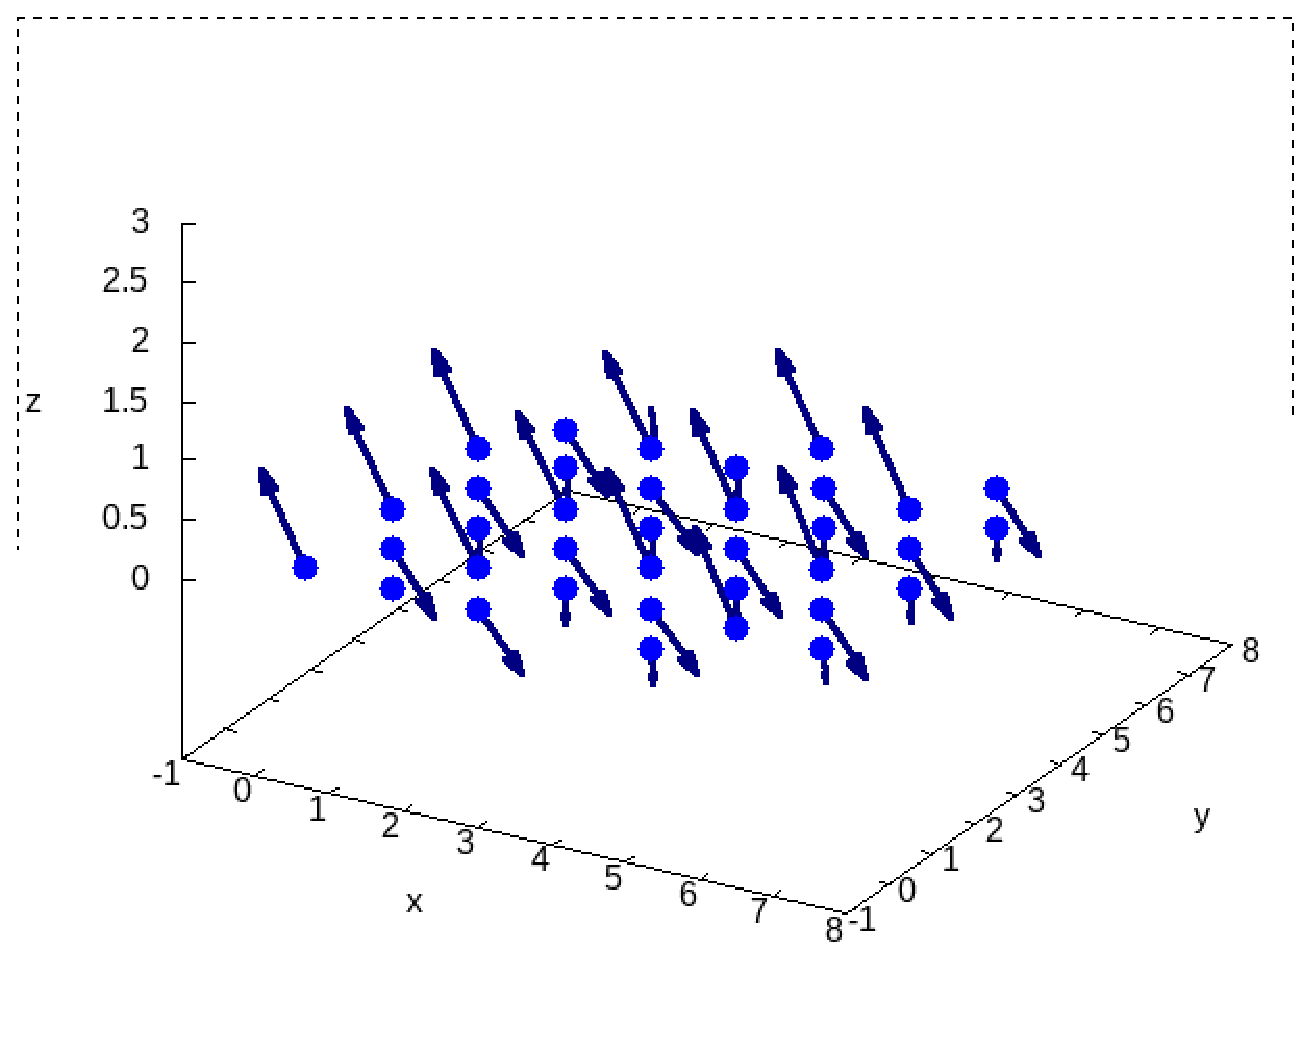
\includegraphics[width=0.5\linewidth]{pictures/AFM013D} \\ б)}
\end{minipage}
\caption{Конечное состояние системы, в которой взаимодействие между спинами носит антиферромагнитный характер $J_0=0.01$, $r_c=2$.}
\label{ris:image5}
\end{figure}
\

\begin{figure}[h]
\begin{minipage}[h]{0.49\linewidth}
\center{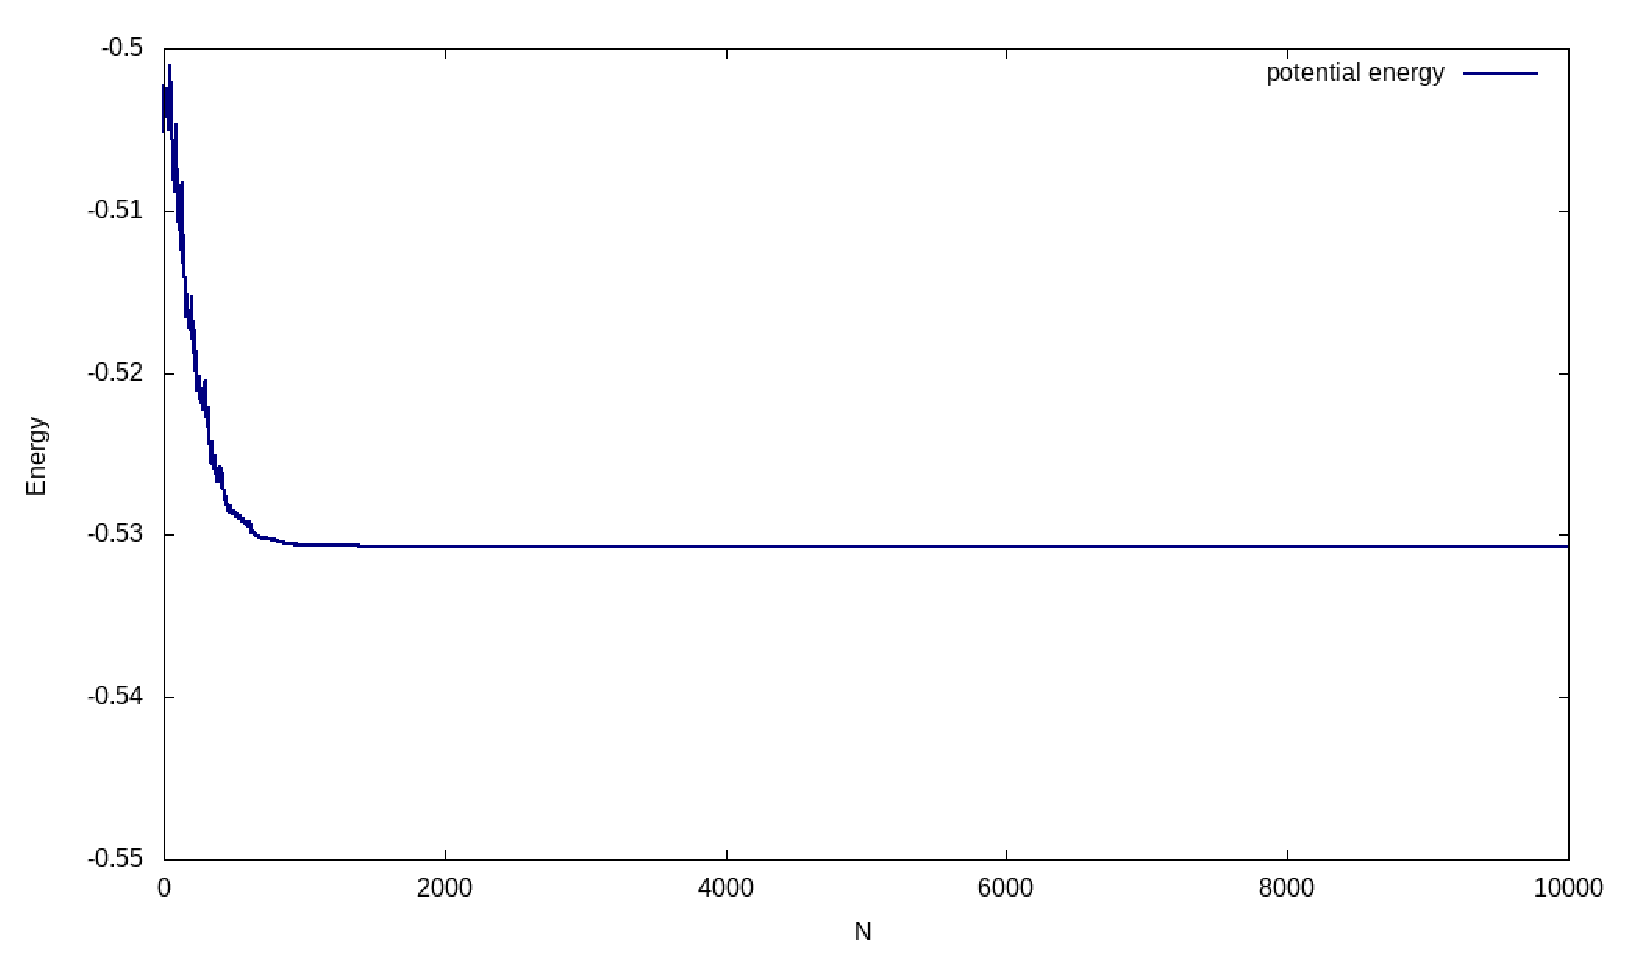
\includegraphics[width=0.5\linewidth]{pictures/energyFM01} \\ а)  FM $J_0=-0.01$, $r_c=2$)}
\end{minipage}
\hfill
\begin{minipage}[h]{0.49\linewidth}
\center{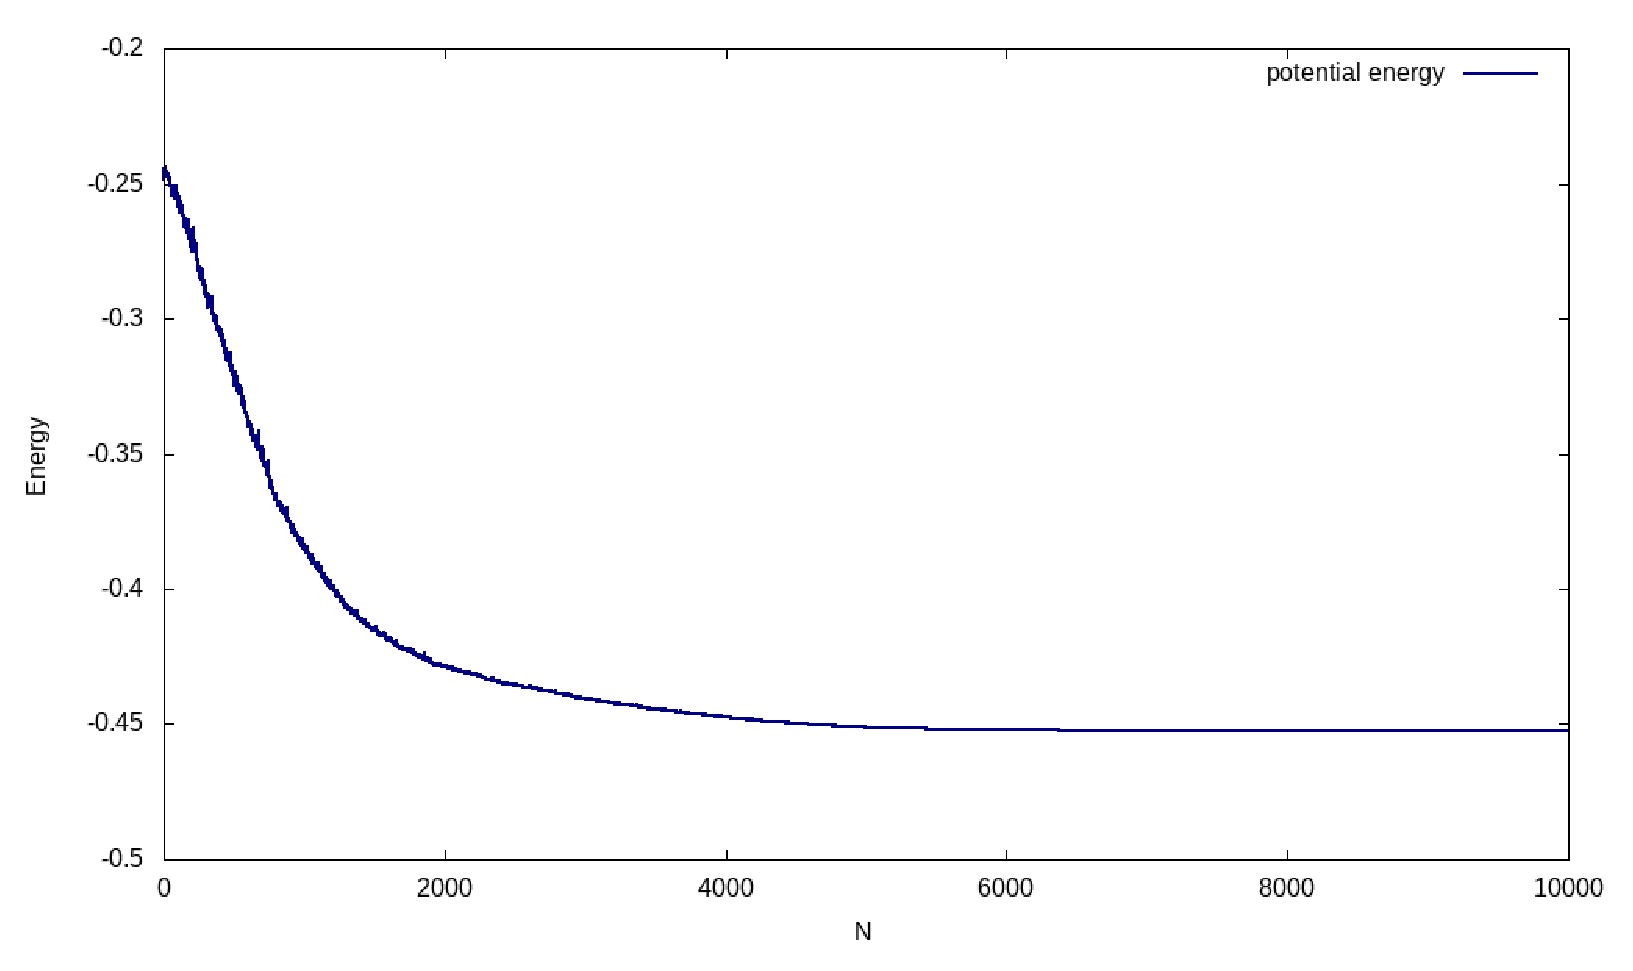
\includegraphics[width=0.5\linewidth]{pictures/energyAFM01} \\ б  AFM $J_0=0.01$, $r_c=2$.)}
\end{minipage}
\caption{График зависимости энергии системы от шага моделирования. }
\label{ris:image6}
\end{figure}
\

\
\newpage
\subsection{$|J_0|=0.1$, $r_c=2$}
Проанализируем поведение систем при различных значениях параметров $J_0$ и $r_c$.
Для начала увеличим $J_0$ на порядок.
На рисунке \ref{ris:image8} и \ref{ris:image9} представлены системы, упорядоченные, соответственно, ферромагнитно и антиферромагнитно после 10000 шагов алгоритма.
\

Из рисунка \ref{ris:image8} можно сделать вывод, что при увеличении $J_0$ на порядок постоянная решетки меняется; при ферромагнитном взаимодействии между спинами решетка остаётся треугольной. 

\
Исходя из состояния системы после моделирования для антиферромагнитного взаимодействия между спинами (рисунок \ref{ris:image9}), можно сделать вывод, что решетки при таких условиях выгоднее прийти в квадратную конфигурацию.


\

\begin{figure}[h]
\begin{minipage}[h]{0.49\linewidth}
\center{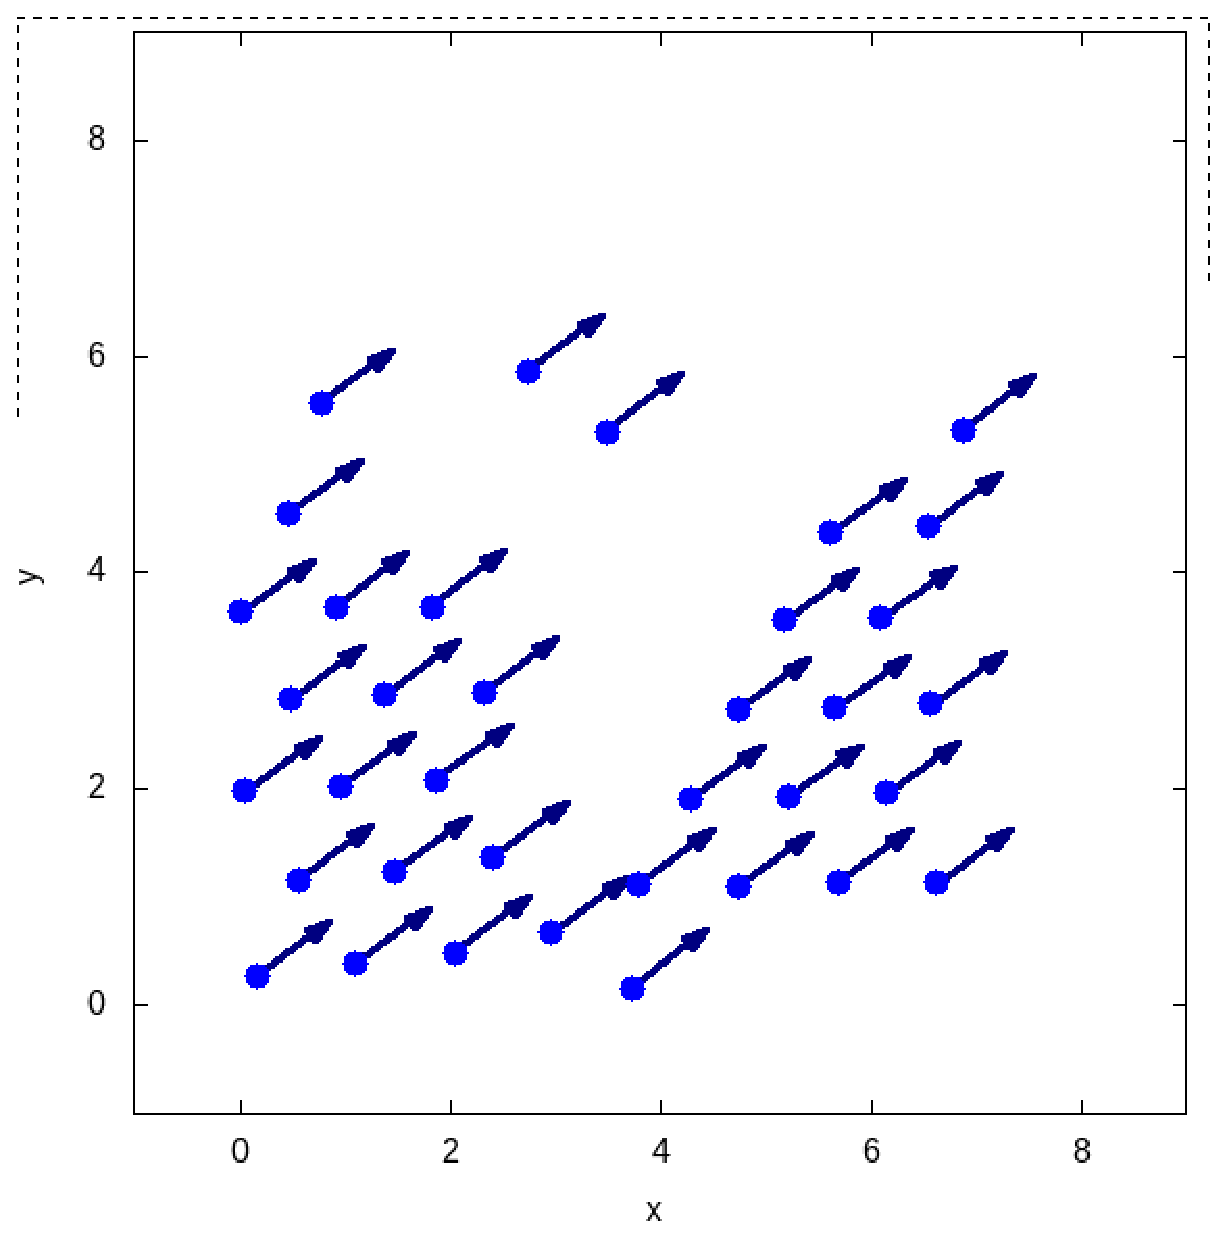
\includegraphics[width=0.5\linewidth]{pictures/FM1} \\ а)}
\end{minipage}
\hfill
\begin{minipage}[h]{0.49\linewidth}
\center{\includegraphics[width=0.5\linewidth]{pictures/FM13D} \\ б)}
\end{minipage}
\caption{Конечное состояние системы, в которой взаимодействие между спинами носит ферромагнитный характер $J_0=-0.1$, $r_c=2$.}
\label{ris:image8}
\end{figure}


\begin{figure}[h]
\begin{minipage}[h]{0.49\linewidth}
\center{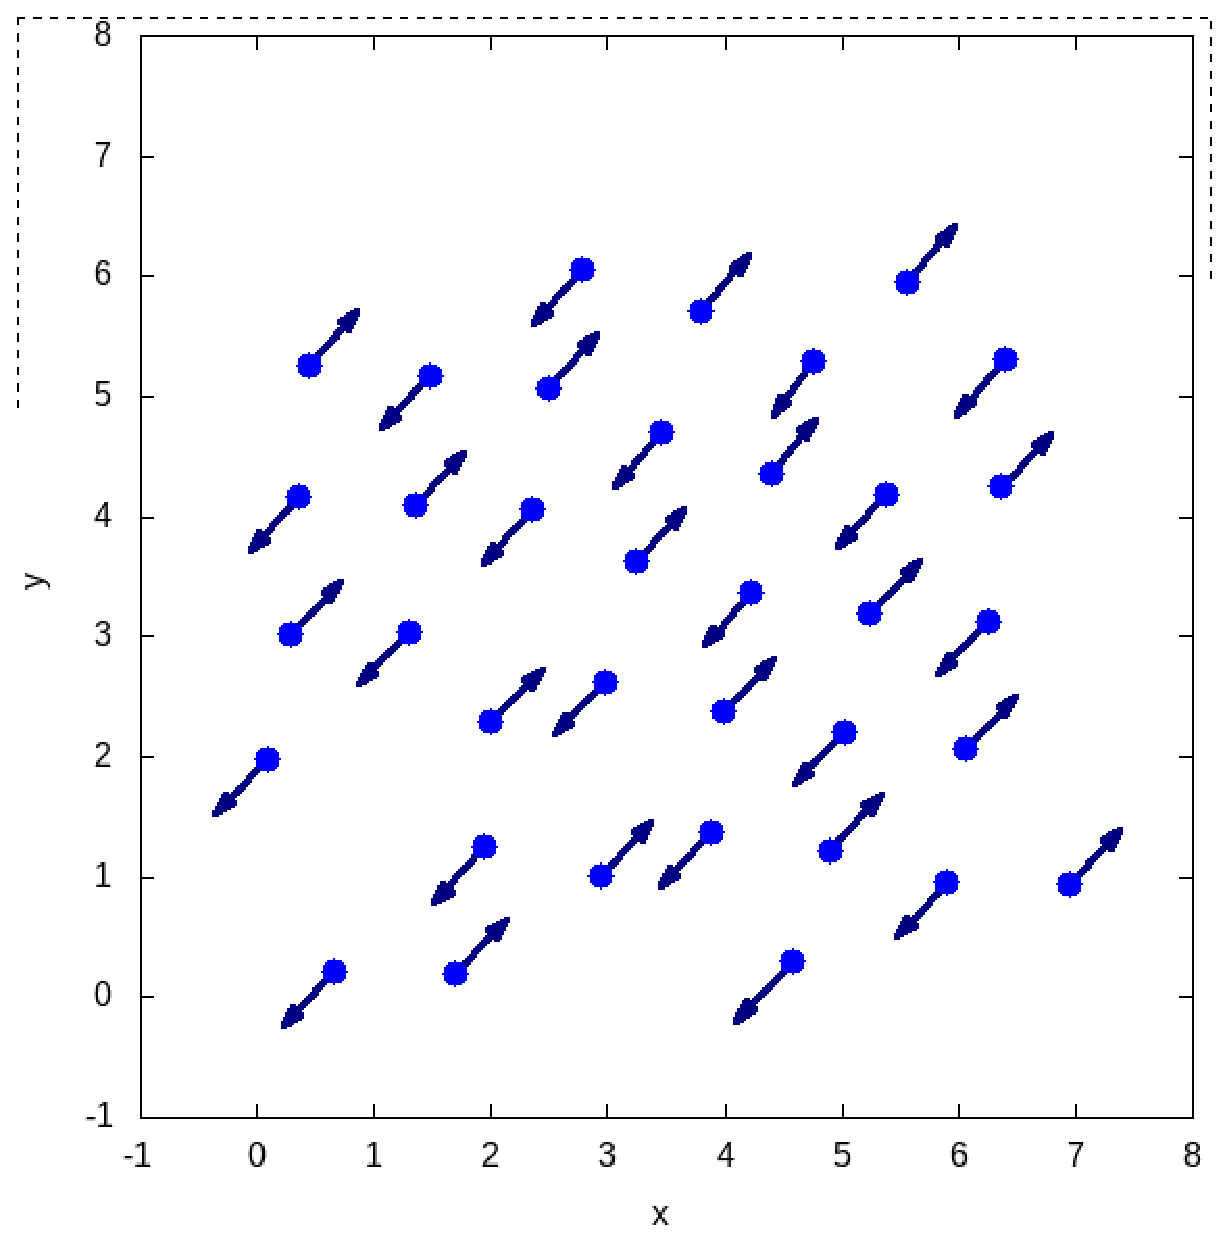
\includegraphics[width=0.5\linewidth]{pictures/AFM1} \\ а)}
\end{minipage}
\hfill
\begin{minipage}[h]{0.49\linewidth}
\center{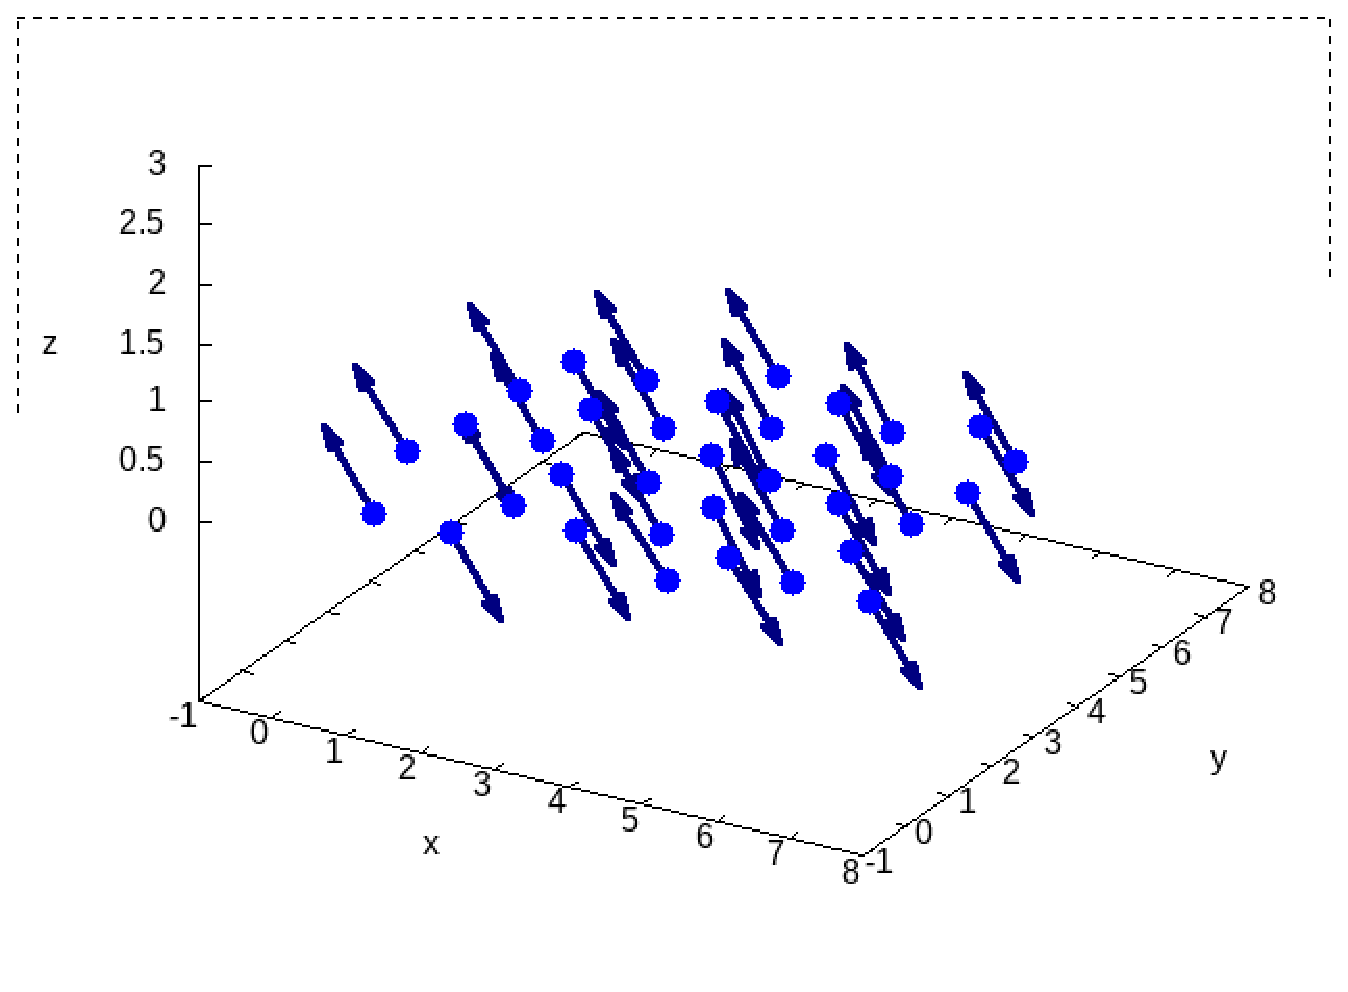
\includegraphics[width=0.5\linewidth]{pictures/AFM13D} \\ б)}
\end{minipage}
\caption{Конечное состояние системы, в которой взаимодействие между спинами носит антиферромагнитный характер $J_0=0.1$, $r_c=2$.}
\label{ris:image9}
\end{figure}


\newpage
\subsection{$|J_0|=0.001$, $r_c=2$}
Далее рассмотрим случай, когда энергия спиновой подсистемы на порядок ниже, то есть выбираем $J_0=0,001$. Конечные состояния систем с ферромагнитным взаимодействием между спинами и антиферромагнитным взаимодействием между спинами представлены, соответственно, на рисунках \ref{ris:image14} и \ref{ris:image16}.
\ 



\begin{figure}[h]
\begin{minipage}[h]{0.49\linewidth}
\center{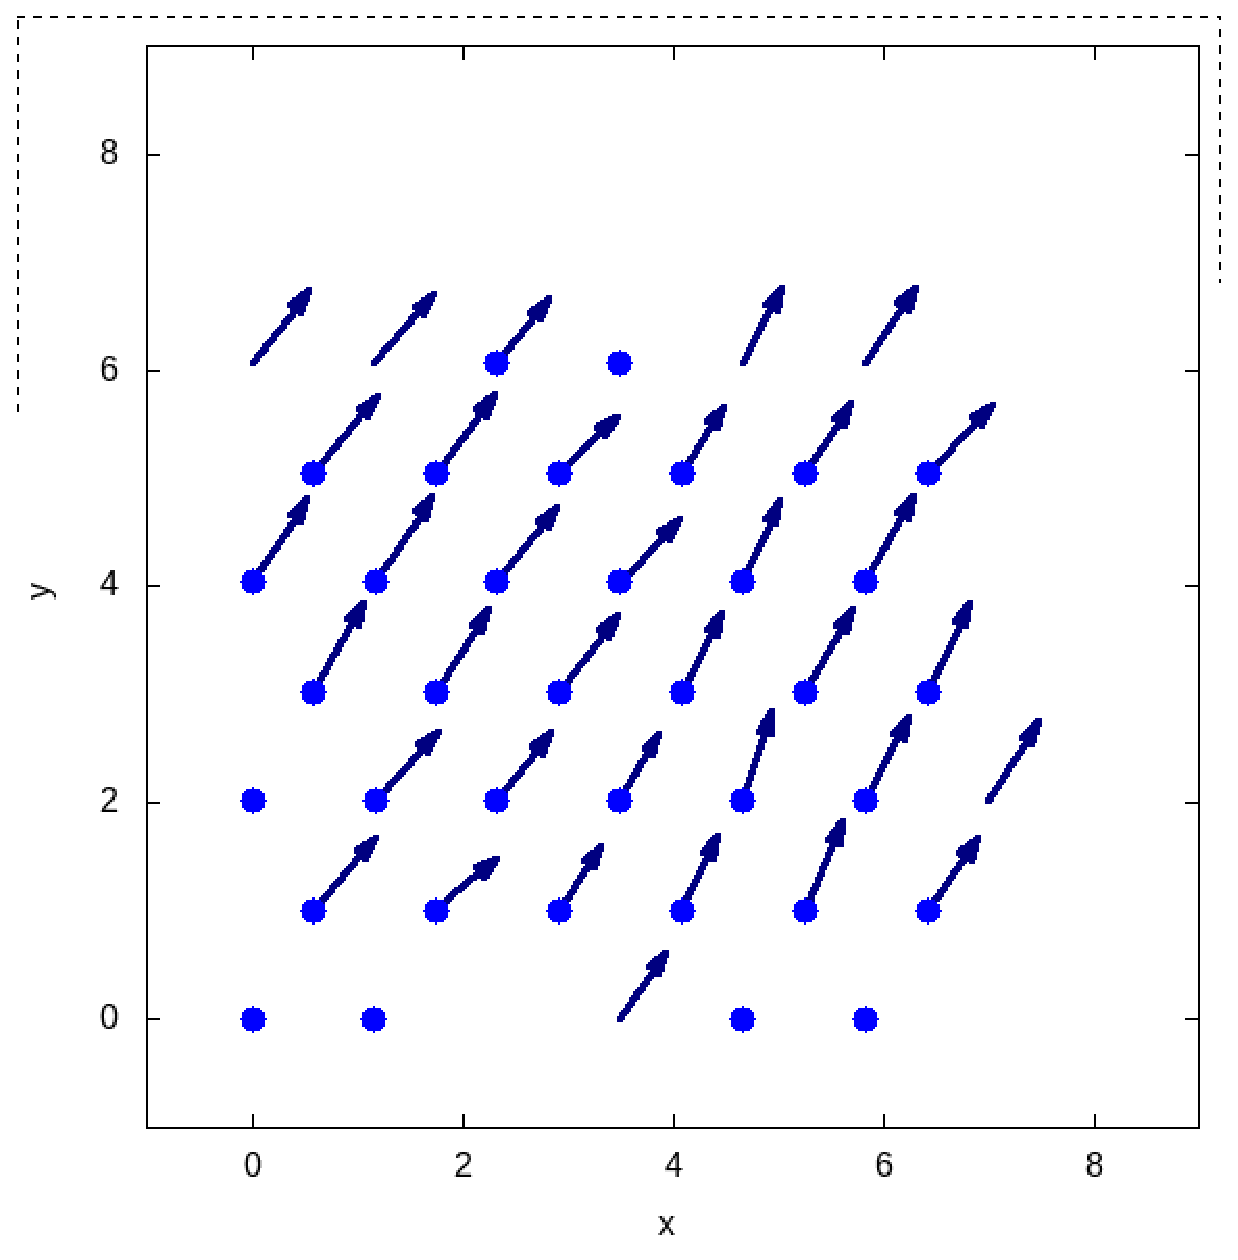
\includegraphics[width=0.5\linewidth]{pictures/FM001} \\ а)}
\end{minipage}
\hfill
\begin{minipage}[h]{0.49\linewidth}
\center{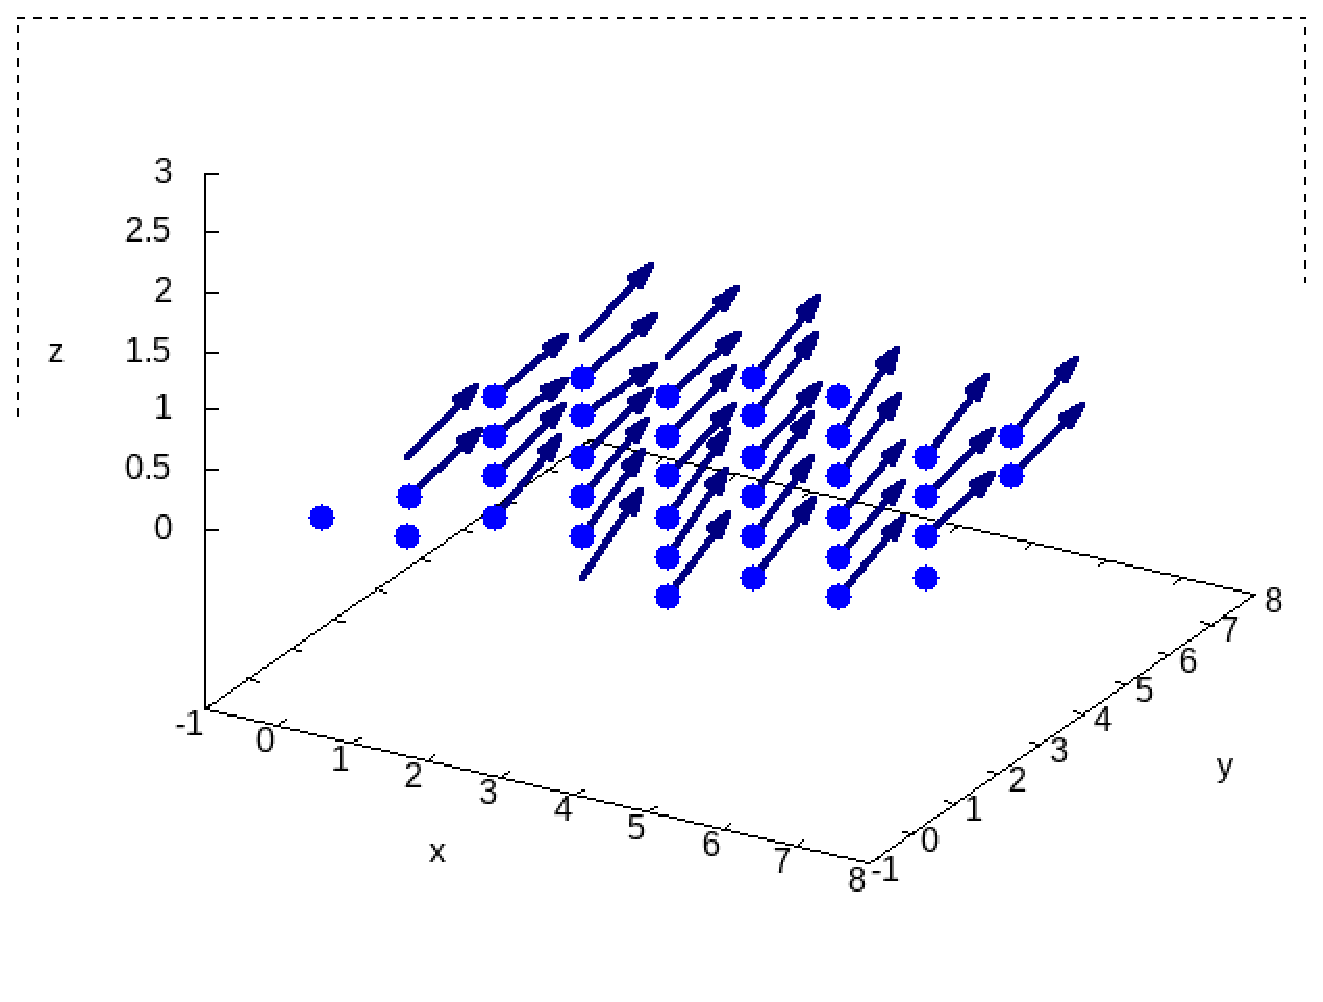
\includegraphics[width=0.5\linewidth]{pictures/FM0013D} \\ б)}
\end{minipage}
\caption{Конечное состояние системы, в которой взаимодействие между спинами носит ферромагнитный характер $J_0=-0.001$, $r_c=2$}
\label{ris:image14}
\end{figure}


\begin{figure}[h!]
\begin{minipage}[h]{0.49\linewidth}
\center{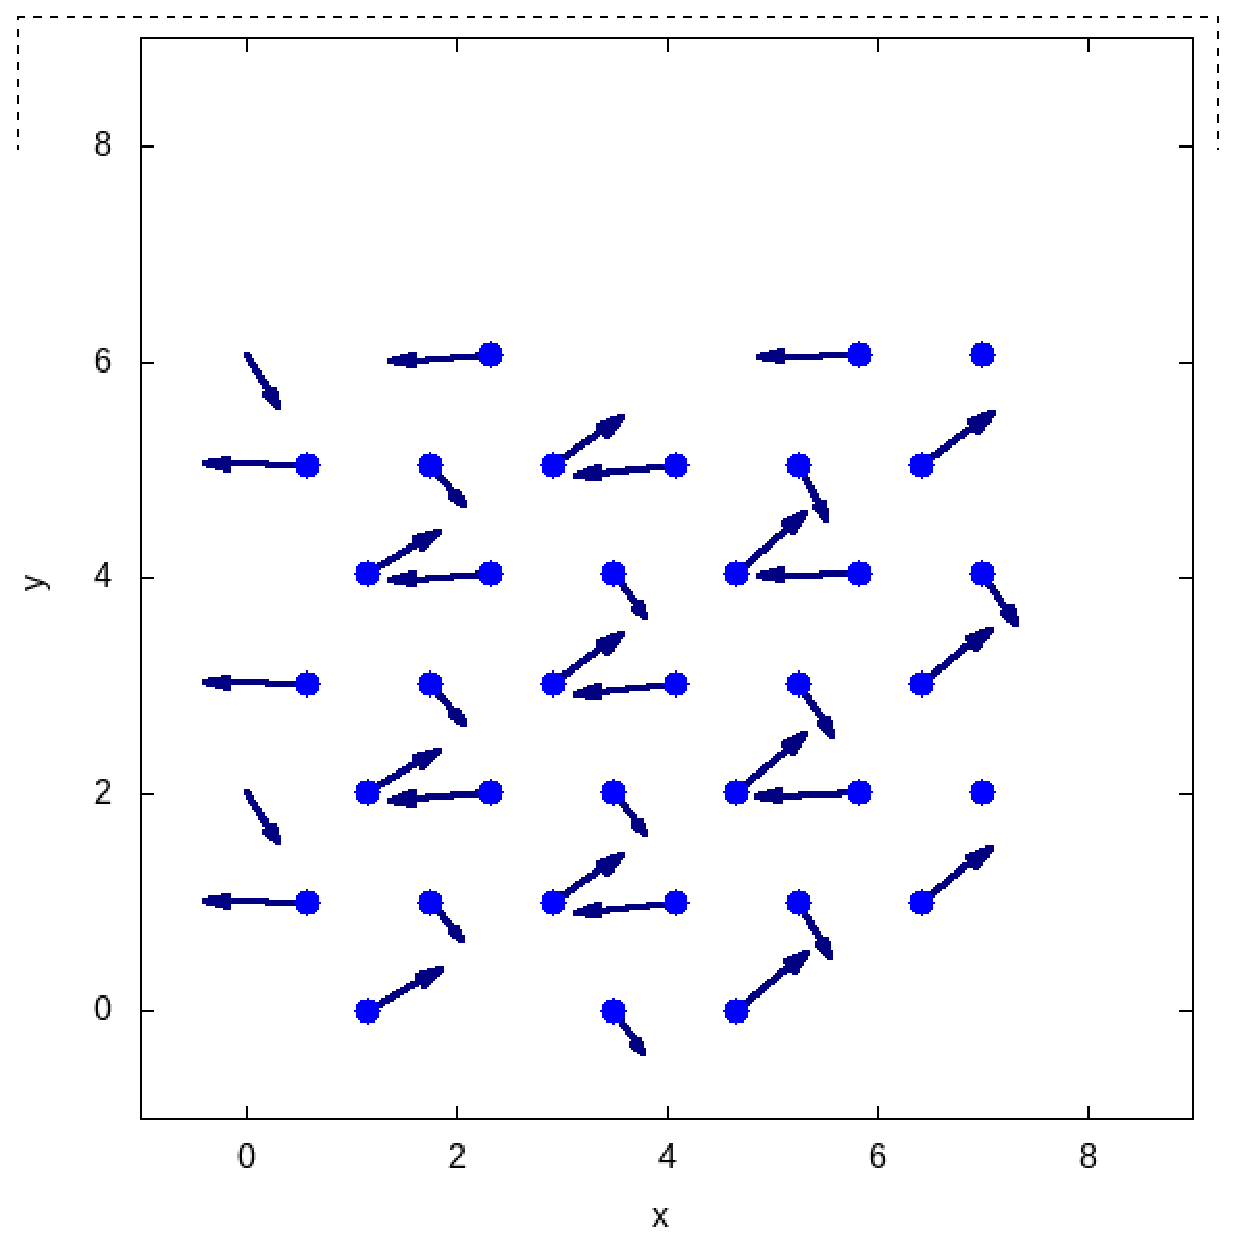
\includegraphics[width=0.5\linewidth]{pictures/AFM001} \\ а)}
\end{minipage}
\hfill
\begin{minipage}[h]{0.49\linewidth}
\center{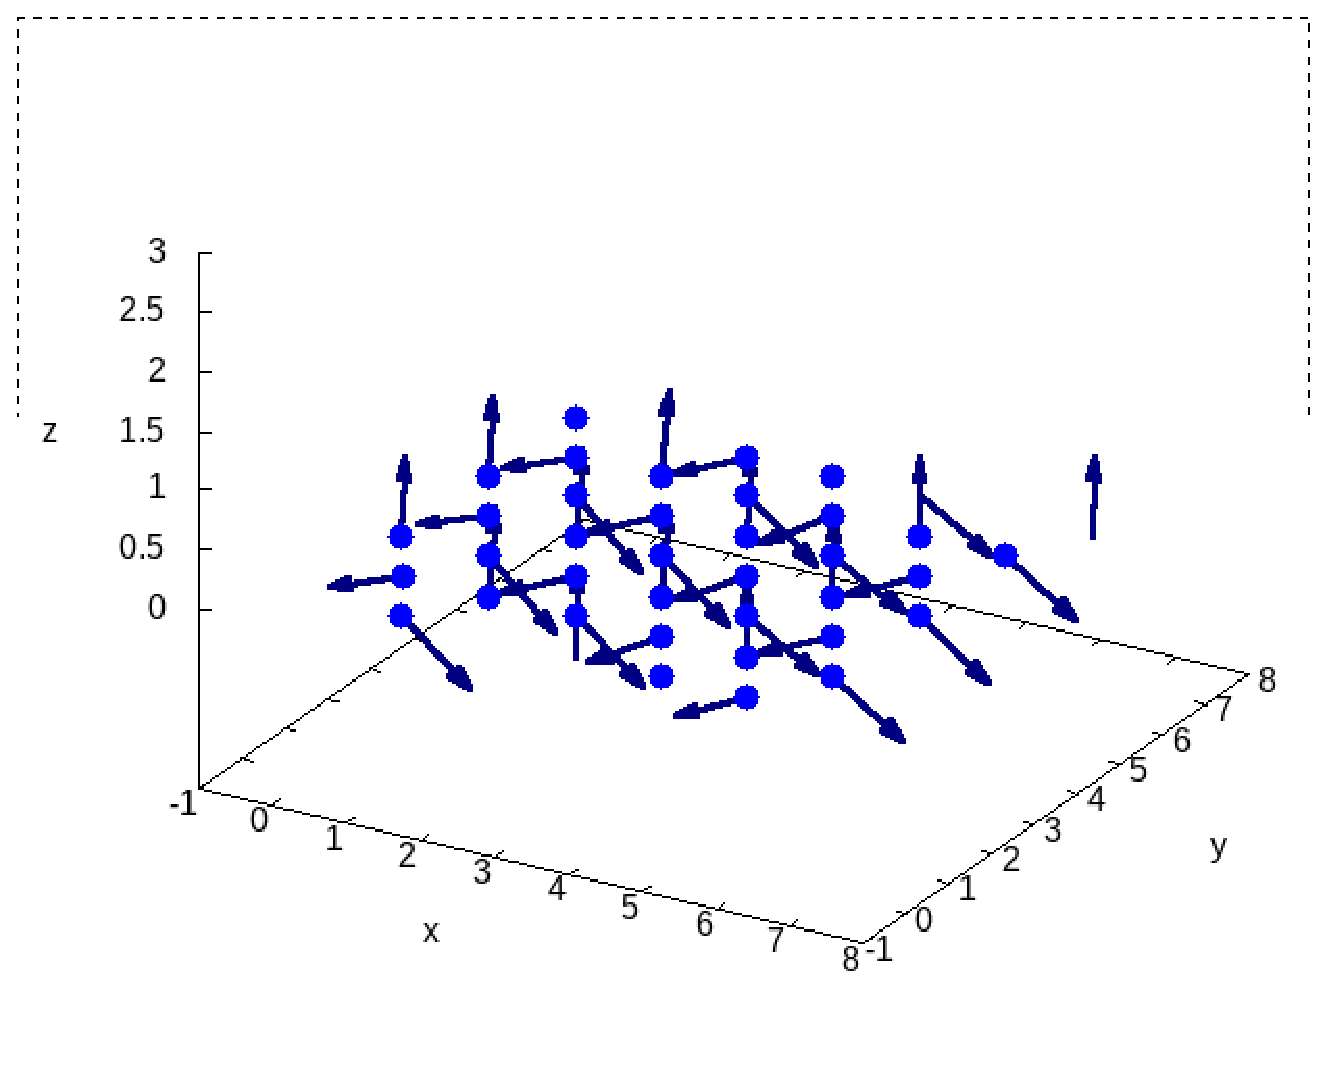
\includegraphics[width=0.5\linewidth]{pictures/AFM0013D} \\ б)}
\end{minipage}
\caption{Конечное состояние системы, в которой взаимодействие между спинами носит антиферромагнитный характер $J_0=0.001$, $r_c=2$}
\label{ris:image16}
\end{figure}


\newpage
\subsection{$|J_0|=0.01$, $r_c=4$}

Теперь вернем параметр $J_0$ к исходному значению $|J_0=0.01|$ и исследуем изменения в поведении систем в зависимости от радиуса обрезки $r_c$. Для значения $r_c$, выбранного меньше постоянной решетки, никакого упорядочения не происходит - спины свободно вращаются в пространстве. Значит, рассмотрим поведение системы для $r_c$, большего, чем постоянная решетки. Соответствующие изображения конечных состояний систем с ФМ и АФМ упорядочением представлены на рисунках, соответственно, \ref{ris:image17} и \ref{ris:image19}.
\

На рисунке \ref{ris:image17} изображено конечное состояние системы с ферромагнитным характером взамодействия между спинами. При увеличении параметра $r_c$ изменений глобальных не произошло, спины упорядочиваются параллельно, что типично для ФМ взаимодействия.


\
\begin{figure}[h]
\begin{minipage}[h]{0.49\linewidth}
\center{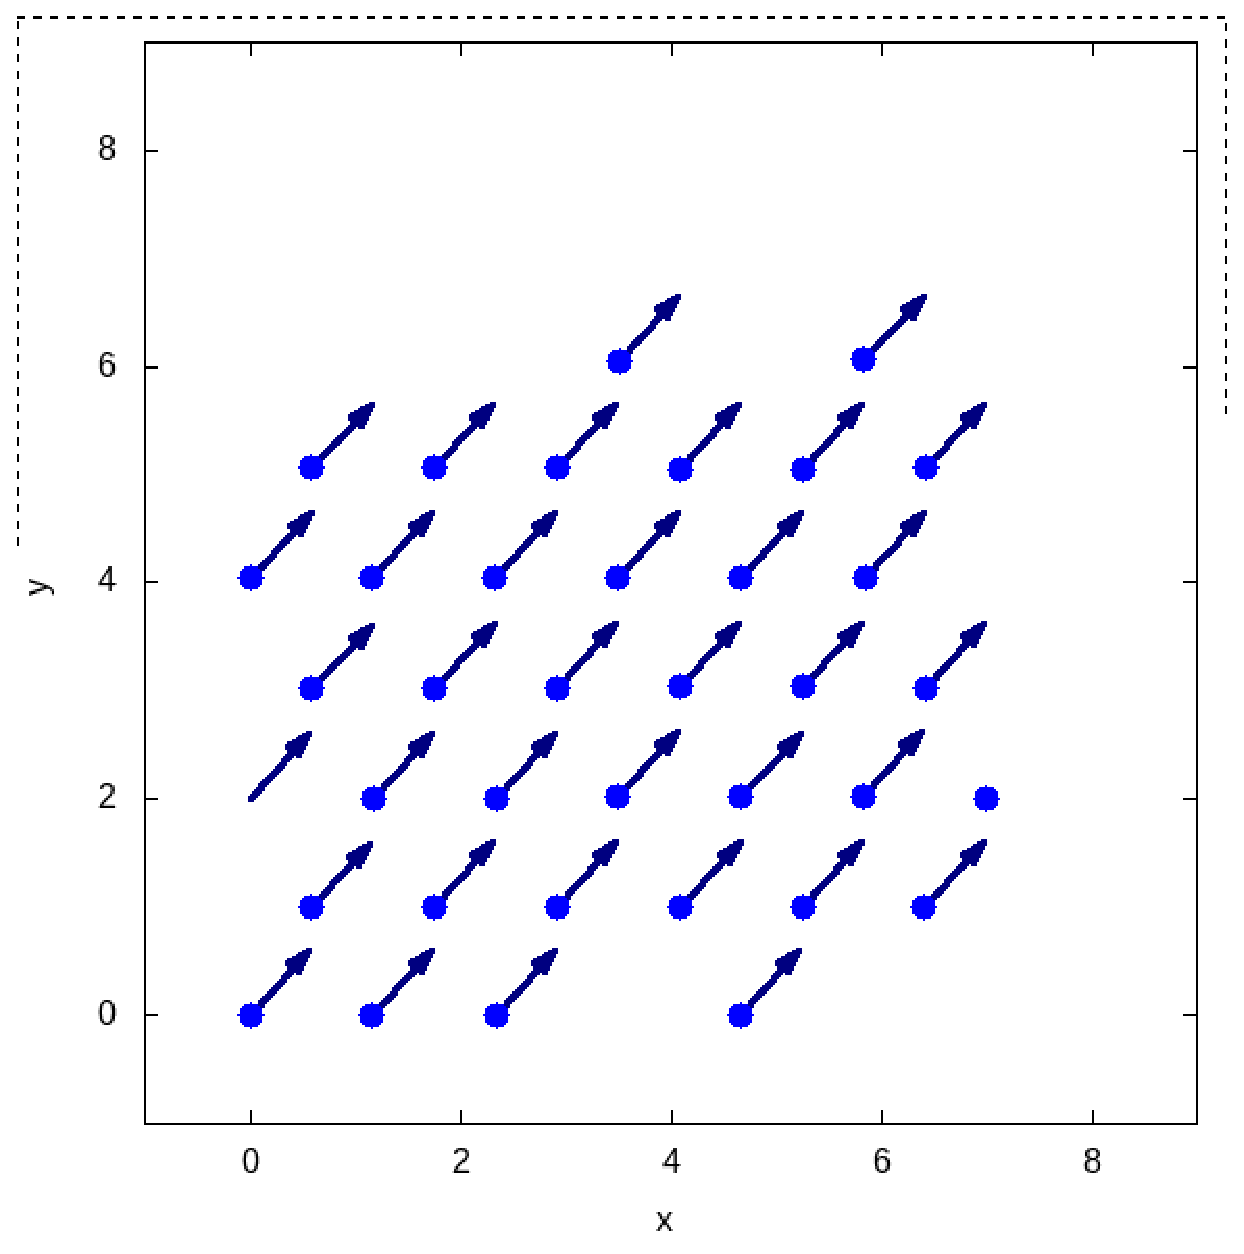
\includegraphics[width=0.5\linewidth]{pictures/FMr4} \\ а)}
\end{minipage}
\hfill
\begin{minipage}[h]{0.49\linewidth}
\center{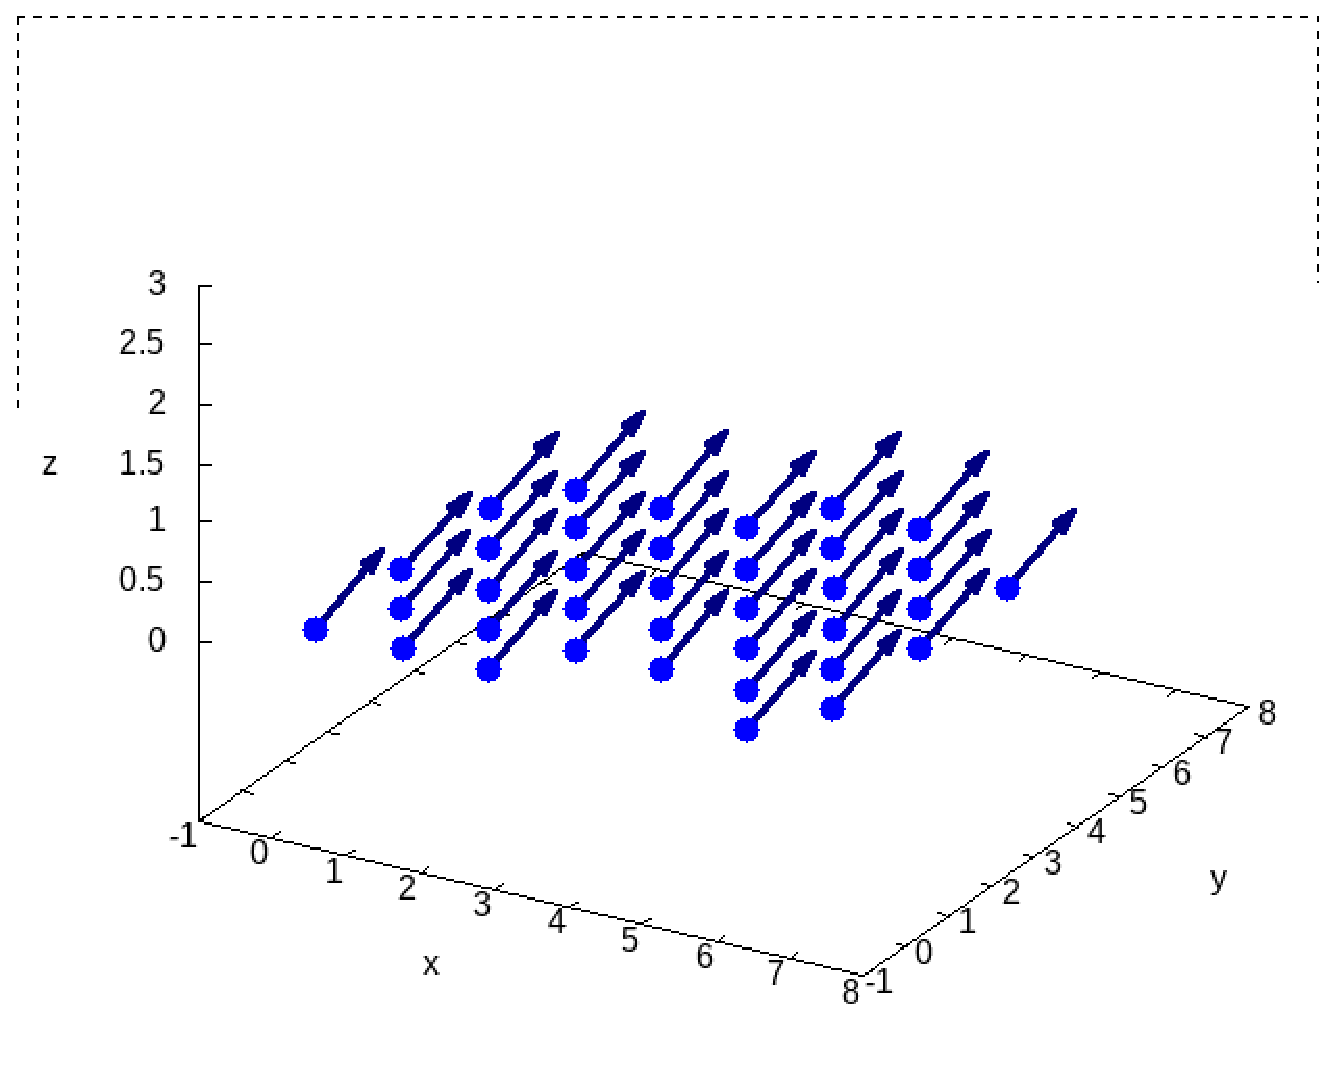
\includegraphics[width=0.5\linewidth]{pictures/FMr43D} \\ б)}
\end{minipage}
\caption{Конечное состояние системы, в которой взаимодействие между спинами носит ферромагнитный характер $J_0=-0.01$, $r_c=4$.}
\label{ris:image17}
\end{figure}



Как видно из рисунка \ref{ris:image19} конечная конфигурация системы, спины которой взаимодействуют антиферромагнитно, отличается от полученных ранее, взаимная ориентация спинов носит более сложный характер.
\

\begin{figure}[h]
\begin{minipage}[h]{0.49\linewidth}
\center{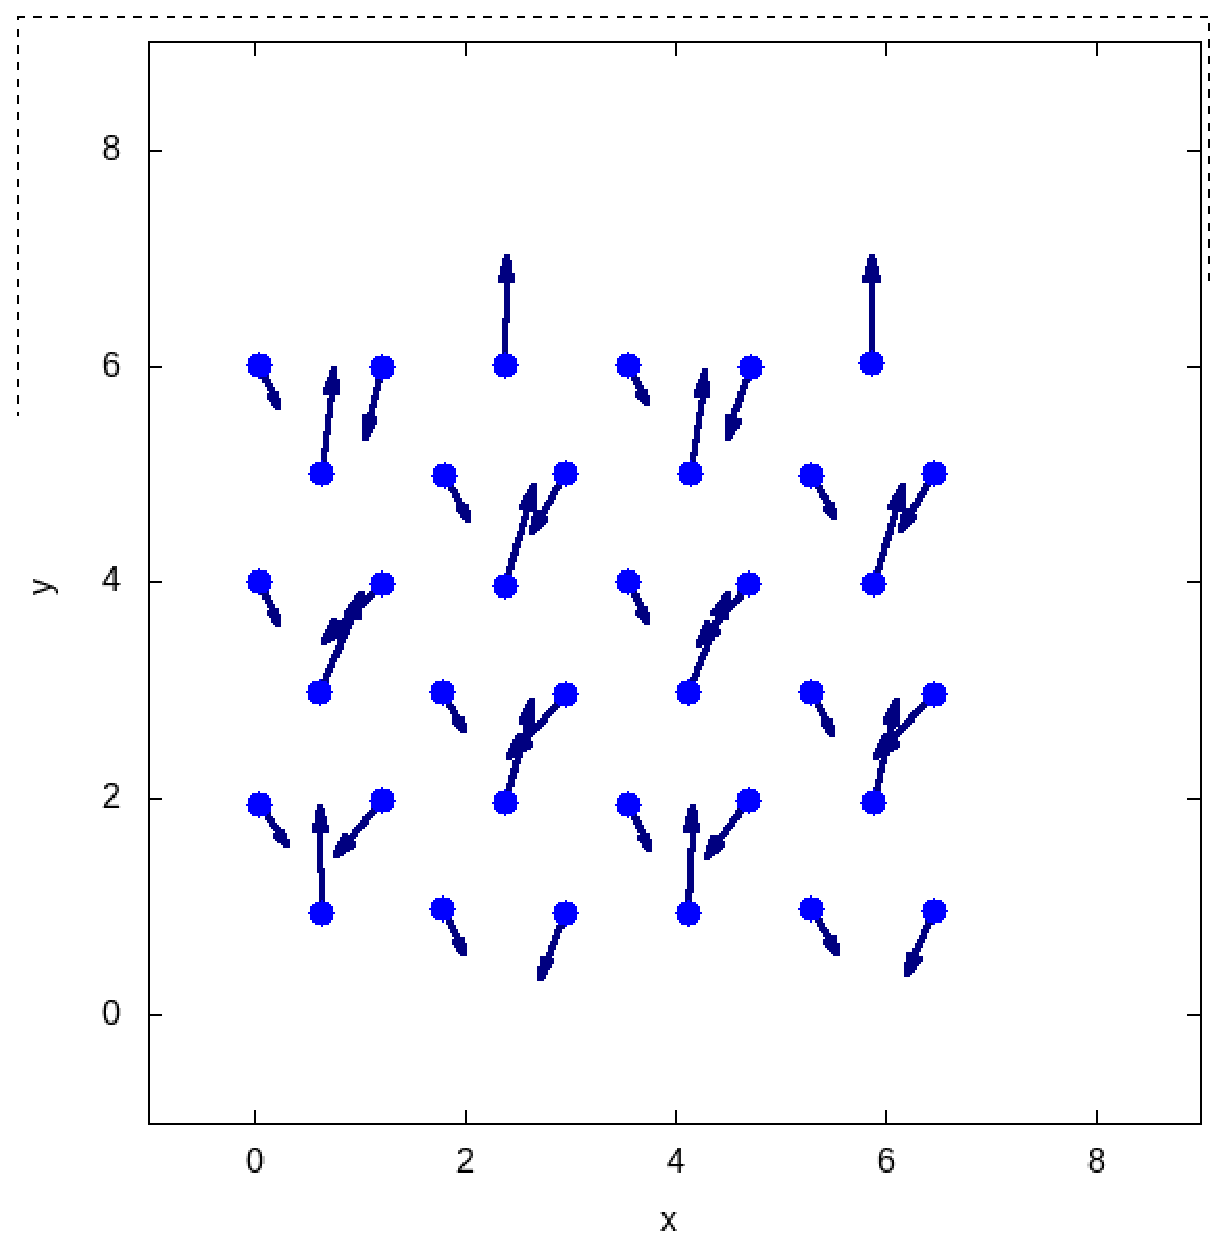
\includegraphics[width=0.5\linewidth]{pictures/AFMr4} \\ а)}
\end{minipage}
\hfill
\begin{minipage}[h]{0.49\linewidth}
\center{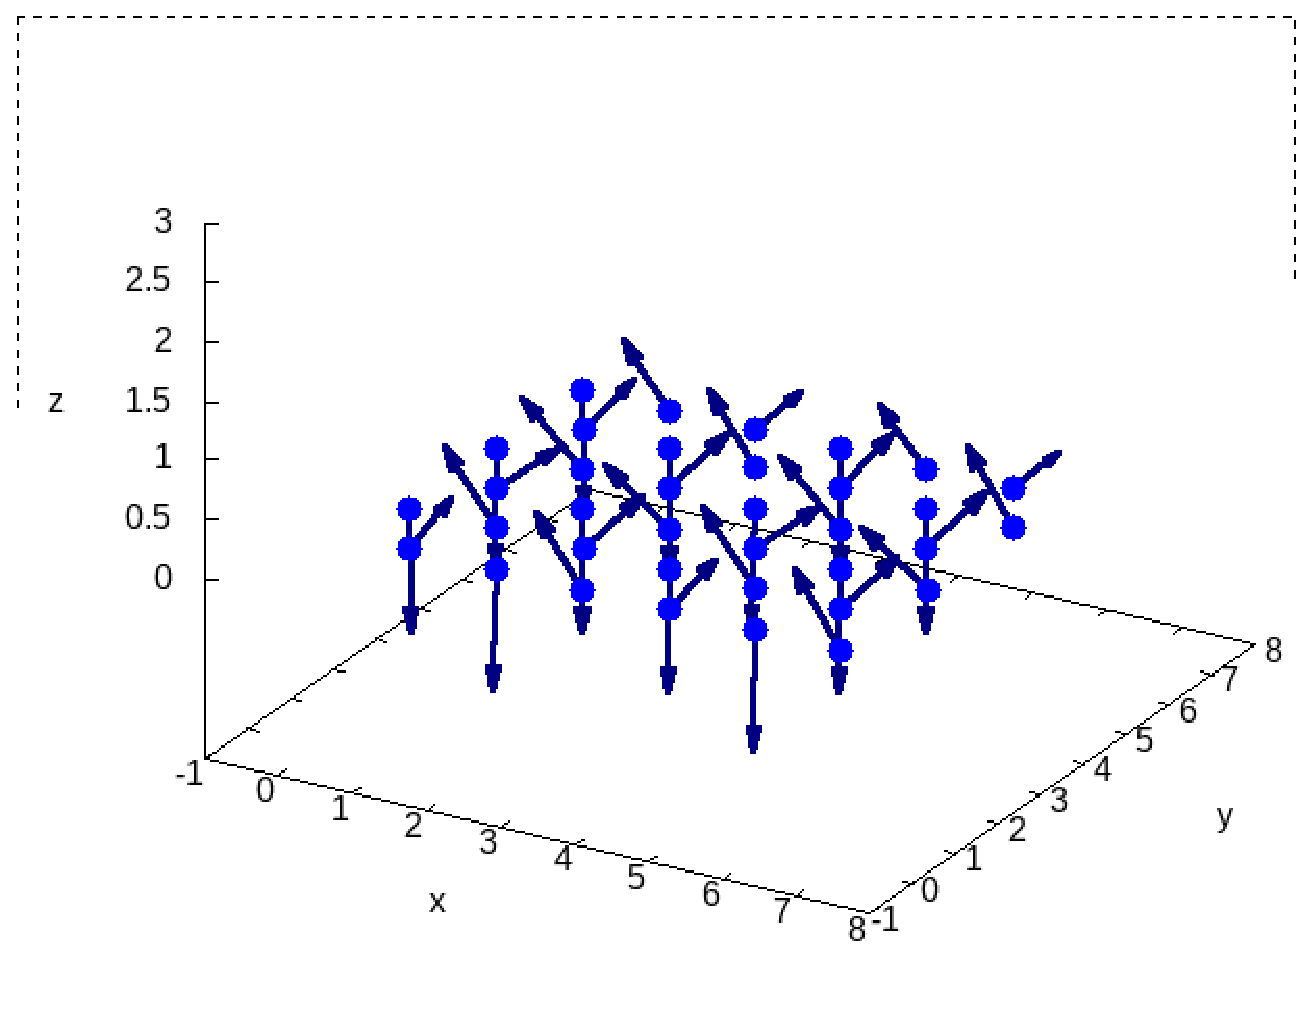
\includegraphics[width=0.5\linewidth]{pictures/AFMr43D} \\ б)}
\end{minipage}
\caption{Конечное состояние системы, в которой взаимодействие между спинами носит антиферромагнитный характер $J_0=0.01$, $r_c=4$.}
\label{ris:image19}
\end{figure}

\newpage
\subsection{Выводы}


В ходе данной работы была разработана программа на языке C++, моделирующая объединенную молекулярную и спиновую динамику при помощи метода Монте-Карло (задействован алгоритм Метрополиса). В молекулярной подсистеме взаимодействия частиц задаются через потенциал Леннарда-Джонса, за взаимодействие спиновой подсистемы отвечает обменное взаимодействие Гейзенберга. Начальное положение частиц системы выбрано в виде треугольно решетки, в которой частицы колеблются вблизи своих положений равновесия.
\

При помощи разработанной программы и пакета GNUplot была проанализирована зависимость поведения систем от двух параметров - $r_c$ и $J_0$. В случае, когда энергетический вклад спиновой подсистемы был равен вкладу молекулярной подсистемы, частицы системы остаются в узлах треугольной решетки, а спины упорядочиваются согласно характеру взаимодействия между ними. В случае, когда вклад в энергию спиновой системы был увеличен, в системе, для спинов характерен антиферромагнитный характер взаимодействия, частицы нашли своё положение равновесия в узлах квадратной решетки; в случае ферромагнитного взаимодействия в минимуме энергии частицы системы выстраивались в узлах треугольной решетки с меньшей постоянной решетки.
В обратном случае, когда преобладал энергетический вклад молекулярной подсистемы, спины упорядочивались не в полной мере.
\
\end{document}